\appendix
\addcontentsline{toc}{part}{\appendixname}

%\begin{appendices}

	\chapter{Instalación y Configuración del software necesario} \label{app:instalacion_software}
		%\chapterimage[width=12cm]{figuras/Portadas_2.png}
		\hrule
		\vspace{3mm}
		\input{anexos/instalacion_software}
	
	\chapter{Listado de piezas diseñadas} \label{app:listadoPiezas}
		\hrule
		\vspace{3mm}
		\completar
\begin{center}
\begin{longtable}{|c|c|c|c|c|c|}
\caption{Listado de piezas diseñadas de fabricación propia}\\
\hline
\textbf{Num} & \textbf{Esquema Pieza} & \textbf{Referencia} & \textbf{Cantidad} & \textbf{Descripción} & \textbf{Peso Estimado}$^1$ \\
\hline
\endfirsthead
\multicolumn{5}{c}%
{\tablename\ \thetable\ -- \textit{Continuación de la página anterior}} \\
\hline
\textbf{Num} & \textbf{Esquema Pieza} & \textbf{Referencia} & \textbf{Cantidad} & \textbf{Descripción} & \textbf{Peso Estimado}$^1$ \\
\hline
\endhead
\multicolumn{5}{l}{\begin{minipage}{.8\linewidth}
	%do not draw the footnoterule
	\footnotesize{$^1$ El peso estimado se obtiene con el programa Cura \completar aplicando los parámetros de la tabla \ref{tab:listadoPiezas:param_impresion}. Este peso incluye el de los soportes necesarios para su impresión.}
\end{minipage}} \\ 
\hline \multicolumn{5}{r}{\textit{Continua en la página siguiente}} \\
\endfoot
\hline
%\insertTableNotes
\endlastfoot
1 & \iconoImagen{Base} & blah & 1  & blah & 193g \\
\hline
2 & \iconoImagen{RailA} & blah & 1 & blah & 24g \\
\hline
3 & \iconoImagen{RailB} & blah & 1 & blah & 24g \\
\hline
4 & \iconoImagen{PoleaMotor} & blah & 2 & blah & 3g \\
\hline
5 & \iconoImagen{EncajeTuboInterior} & blah & 1 & blah & 54g \\
\hline
6 & \iconoImagen{EncajeTuboExterior} & blah & 1 & blah & 128g \\
\hline
7 & \iconoImagen{FijacionBarraPieB} & blah & 1 & blah & blah \\
\hline
8 & \iconoImagen{FijacionBarraPie} & blah & 1 & blah & blah \\
\hline
10 & \iconoImagen{RuedaMotorGiroZ} & blah & 1 & blah & 18g \\
\hline
19 & \iconoImagen{AdaptadorPoleaNegra} & blah & 2 & blah & 1g \\
\hline
19 & \iconoImagen{AdaptadorPoleaNegra} & \completarCon{SeparadorPoleas} & 2 & blah & 20g \\
\hline
9 & \iconoImagen{SoportePlaca} & blah & 1 & 10g \\
\hline
11 & \iconoImagen{UnionBarrasIntermediasA} & blah & 1 & blah & blah \\
\hline
12 & \iconoImagen{UnionBarrasIntermediasB} & blah & 1 & blah & blah \\
\hline
13 & \iconoImagen{RuedaTransmisionSuperior} & blah & 1 & blah & 8g \\
\hline
14 & \iconoImagen{TapaPotenciometro} & blah & 1 & blah & blah \\
\hline
15 & \iconoImagen{EngranajePotenciometro} & blah & 1 & blah & blah \\
\hline
16 & \iconoImagen{EngranajeBarra} & blah & 1 & blah & blah \\
\hline
17 & \iconoImagen{UnionBarrasSuperiorA} & blah & 1 & blah & blah \\
\hline
18 & \iconoImagen{PoleaColumpioRedir} & blah & 3 & blah & blah \\
\hline
19 & \iconoImagen{CubrePoleaColumpio} & blah & 2 & blah & 6g \\
\hline
20 & \iconoImagen{CubrePoleaColumpioB} & blah & 2 & blah & blah \\
\hline
21 & \iconoImagen{CubrePoleaRedireccionB} & blah & 1 & blah & blah \\
\hline
22 & \iconoImagen{CubrePoleaRedireccion} & blah & 1 & blah & blah \\
\hline
23 & \iconoImagen{PiezaRodamientosSandwich} & blah & 2 & blah & 39g \\
\hline
24 & \iconoImagen{PiezaRodamientosSandwichB} & blah & 1 & blah & 39g \\
\hline
25 & \iconoImagen{PiezaRodamientosSandwichPotenciometro} & blah & 1 & blah & 44g \\
\hline 
26 & \iconoImagen{TapaPotenciometroA2} & blah & 1 & 1 & 2g \\
\hline
27 & \iconoImagen{PiezaMetacrilato} & blah & 2 & blah & - \\
\hline
28 & \iconoImagen{PiezaUnionSandwich} & blah & 4 & blah & 9g \\
\hline
29 & \iconoImagen{RealimentacionSandwich} & blah & 1 & blah & 24g \\
\hline
30 & \iconoImagen{SandwichAcoplamientoRodamientoBarra} & blah & 1 & blah & blah \\
\hline
\end{longtable}

\end{center}


\begin{center}
\begin{table}[H]
    \caption{Parámetros de las piezas para la estimación de peso}
    \label{tab:listadoPiezas:param_impresion}
    \begin{minipage}{\textwidth}
    \begin{tabular}{ |c|c|c|c| }
    \hline
    a & a & a & a \\ 
    %1 & \iconoImagen{Base}{0.2} & blah & \completar \\
    \hline
    \end{tabular}
    \end{minipage}
\end{table}
\end{center}

	
	\chapter{Montaje del prototipo} \label{app:montajePiezas}
		\hrule
		\vspace{3mm}
		Complementando a la lista de figuras presentada en el anexo \ref{app:listadoPiezas} se adjuntan a continuación unas nociones sobre como se ensambla el prototipo. Se espera que las diferentes imágenes permitan ubicar en el diseño las diferentes piezas descritas.
		
		\begin{landscape}
		    	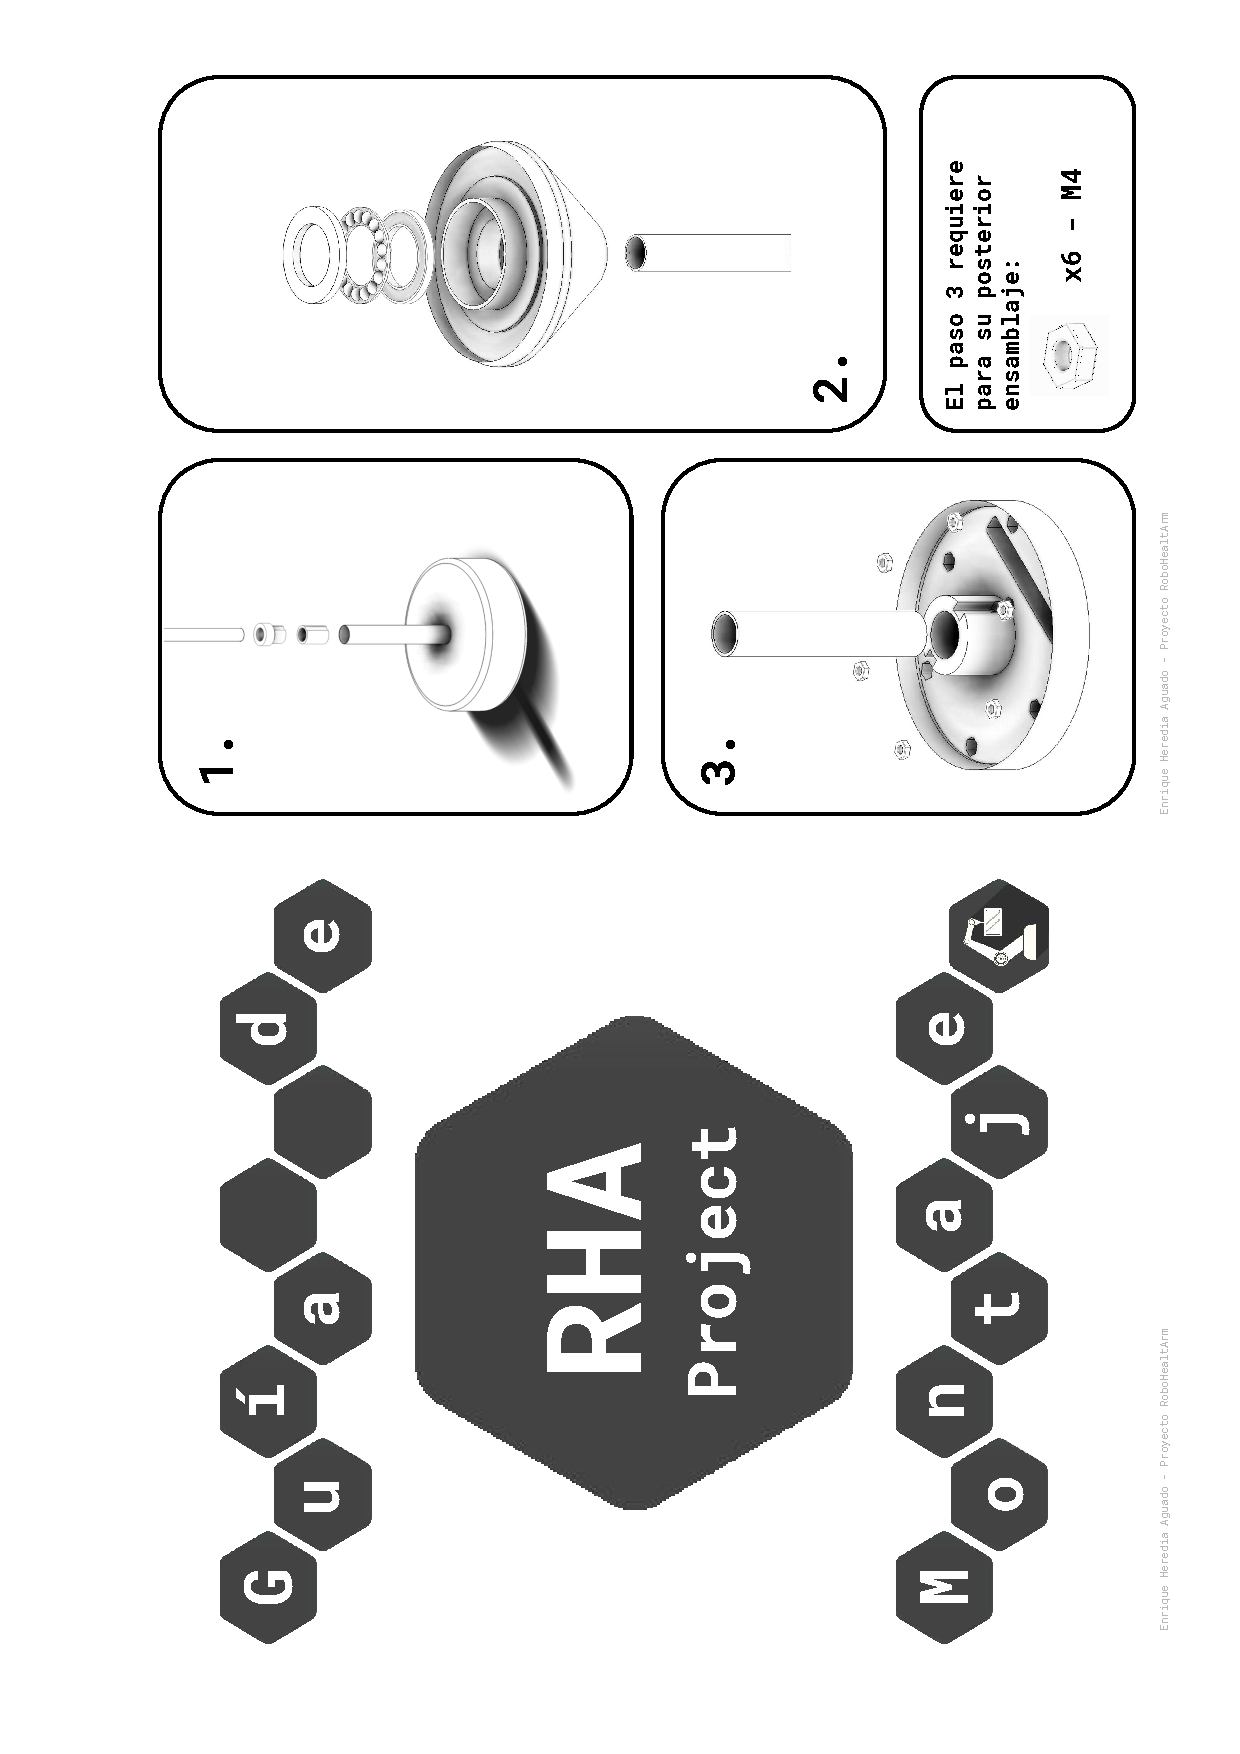
\includepdf[pages=-]{figuras/EnsamblajeRHA.pdf}
		\end{landscape}
	
	\chapter{Reglas de codificación del Software} \label{app:codificacionSW}
		\hrule
		\vspace{3mm}
		Las reglas de codificación aplicadas al software del proyecto se han obtenido, por utilizar una referencia, de las reglas aplicadas por Google en sus proyectos libres. Esta guía está ampliamente documentada en \cite{googlecppguide} e incluye su propia herramienta para comprobar su correcta aplicación, Cpplint, lo que facilita la revisión del código así como corrección de desviaciones de estilo.
\\

En este anexo se traducen y resumen los aspectos más importantes de dicha guía. En algunos casos se han adaptado las reglas al caso concreto de este proyecto.
\\

Establecer unas reglas de codificación, unificando un estilo en la notación y uso de la sintaxis, es interesante de cara a posibilitar una mayor facilidad de lectura en futuros desarrollos aumentando así la mantenibilidad del código.

Estas reglas aplican al código C++ del proyecto, no a los \ingles{scripts} auxiliares.

\section{Aspectos generales} \label{sec:codificacionSW:general}

\section{Ficheros de cabecera} \label{sec:codificacionSW:cabeceras}

    En general todos los ficheros con extensión \codigo{.cpp} correspondientes a las librerías deberán ir acompañados del fichero de cabecera \codigo{.h} correspondiente.
    \\
    
    Quedan exentos de cumplir esta regla los ficheros correspondientes a Test (unitarios, de integración, etc) así como ficheros que contengan únicamente una función \codigo{main()}.

\minititulo{Inclusión Múltiple}

    Para evitar problemas de inclusión múltiple todos los ficheros de cabecera con extensión \codigo{.h} deberán incluir guardas con el siguiente formato y escrito en mayúsculas: \codigo{<nombre\_del\_fichero>\_<extensión>. } 
    \\ 
    
    \lstset{language=C, breaklines=true, basicstyle=\footnotesize}
    %Introducir label y caption
    \begin{lstlisting}[frame=single]
Ejemplo:

    #ifndef SERVO_RHA_H
    #define SERVO_RHA_H
    ...
    ...
    ...
    #endif
    \end{lstlisting}
    
\minititulo{Orden de inclusión de ficheros}

    Para evitar problemas en las dependencias de las distintas librerías se incluirán las mismas dejando para el final las librerías propias del proyecto e incluyendo el resto de la más general a la más particular. 
    \\ 
    
    \lstset{language=C, breaklines=true, basicstyle=\footnotesize}
    %Introducir label y caption
    \begin{lstlisting}[frame=single]
Ejemplo orden al incluir cabeceras:

    #include <stdint.h>    // lib estandar de c++
    #include <Arduino.h>     // lib de Arduino
    #include <SoftwareSerial.h>     // lib para controlar el puerto serie. Basado en Arduino
    
    #include "debug.h"     // def y control de las funciones de debug
    #include "rha_types.h"     // tipos de datos
    #include "joint_rha.h"     // clase a incluir
    \end{lstlisting}
    
    Nota: def. se utiliza de aquí en adelante como abreviatura de \ingles{definición}.
    
    Se deben incluir todos los ficheros que definan los símbolos utilizados en el fichero sobre el que se incluyen. Las declaraciones anticipadas de objetos no están permitidas salvo excepciones justificadas.
 
\section{Ámbitos}\label{sec:codificacionSW:ambitos}
\minititulo{Espacios de nombres}

    Como norma general las constantes, variables o funciones que no estén contenidas en ningún objeto se incluirán dentro de un espacio de nombres o \ingles{namespace} que haga referencia a la utilidad de las mismas.
    \\ 
    
    No está permitido usar directivas del tipo \codigo{ <using namespace \_\_\_\_;>.}
    \\ 
    
    Los espacios de nombres se escriben con la primera letra de cada palabra, en caso de haber más de una, en mayúscula y sin separación de ningún tipo.
    \\ 
    
    \lstset{language=C, breaklines=true, basicstyle=\footnotesize}
    %Introducir label y caption
    \begin{lstlisting}[frame=single]
Ejemplo: Constantes referentes al test de comportamiento ante una entrada tipo rampa

    namespace SlopeTest {
        #define SAMPLE_SLOPE 110
        #define SAMPLE_TEST_SLOPE 20
        #define SLOPE_SPEED 0.1
    }
    
Prohibido el uso de:
    
    using namespace StepTest;
    \end{lstlisting}
    
\minititulo{Variables Locales}

    Las variables se definirán preferiblemente en el ámbito más local en que se vayan a utilizar. Preferiblemente la inicialización de las mismas se hará junto a la declaración.
    \\ 
    
    Se pueden dar excepciones, como pueden ser vectores sobre los que se iterará dentro de un bucle u otros casos similares. En estos casos se de declarará el objeto fuera del propio ámbito para evitar recursivas llamadas a constructor y destructor de los mismos.
    \\ 
    
    \lstset{language=C, breaklines=true, basicstyle=\footnotesize}
    %Introducir label y caption
    \begin{lstlisting}[frame=single]
Ejemplo: 
    
    // Siempre que la variable sobre la que se itera no se vaya a utilizar para posteriores operaciones: 
    for(int i = 0, i < 10; i++) {
    }
    
    //mejor que el caso siguiente, que adicionalmente incumple la regla preferente de inicializar la variable cuando se declara:
    int i; 
    for(i = 0, i < 10; i++) {
    }
    
    //queda permitido declarar vectores u otros objetos similares antes si se va a iterar o trabajar sobre los mismos
    int vector[5] = {1,2,3,4,5};
    for(int i = 0, i < 10; i++) {
        Serial.print(vector[i]);
    }

    \end{lstlisting}
    
\section{Clases}\label{sec:codificacionSW:clases}

\minititulo{Constructores y métodos de Inicialización}

Para todos los objetos debe haber constructores por defecto sin parámetros de entrada. Aunque se pueden añadir constructores que inicialicen los diferentes parámetros será obligatorio generar métodos que los inicialicen una vez construido el objeto así como constructores por defecto para todos los métodos. Arduino, aún estando basado en el lenguaje \codigo{C++} no permite un uso completo de memoria dinámica. Los objetos se declaran como miembros haciendo uso del constructor por defecto para ser inicializados posteriormente.
\\ 

    \lstset{language=C, breaklines=true, basicstyle=\footnotesize}
    %Introducir label y caption
    \begin{lstlisting}[frame=single]
Ejemplo: 
    
	//NO se permite:
    - joint_rha.h -
    ServoRHA servo_*;
    - joint_rha.cpp -
    servo_ = new ServoRHA(1, 10, 5);
    
    //Se llama al constructor del objeto para luego inicializarlo:
    - joint_rha.h -
    ServoRHA servo_;
    - joint_rha.cpp -
    servo.init(... params ...);

    \end{lstlisting}

Para evitar funciones con muchos parámetros que reduzcan la legibilidad del código se permite generar diferentes inicializadores para los distintos parámetros. En la documentación del objeto deberá quedar bien claro que inicializadores deben invocarse para el correcto funcionamiento del mismo.

\minititulo{Estructuras o Clases}

Por norma general las estructuras se utilizarán exclusivamente para objetos pasivos, objetos que contienen información. Todo lo demás se codificará dentro una clase.
\\ 

En el caso de estructuras se permiten únicamente métodos para el manejo de los datos sin añadir ninguno tipo de comportamiento, están permitidos los constructores, destructores, métodos de reset, validación, etc. El acceso a los miembros de la estructura se hará directamente sobre los propios parámetros y no mediante métodos específicos. Los parámetros serán siempre públicos para ser consistente con este punto.
\\ 

Para mayores funcionalidades se generará una clase.

\minititulo{Control de Acceso}

Como norma general se declararan como privados todos los atributos de las clases exceptuando aquellos objetos que a su vez tengan, internamente, control de acceso definido (otras clases). De cara a generar Test con clases propias se permite la declaración de atributos como \codigo{protected}.

\section{Tipos de datos}\label{sec:codificacionSW:datos}

Los tipos de datos usados irán acordes con la librería \codigo{stdint.h}. Estos son del tipo \codigo{int16\_t}, \codigo{uint32\_t}, etc. Este tipo de datos garantiza el control del tamaño del dato declarado.

Se utilizarán los nombres \codigo{float} y \codigo{double} convencionales para declarar datos en coma flotante.

\section{Nombres}\label{sec:codificacionSW:nombres}

\minititulo{Reglas generales}

Los nombres deberán ser descriptivos. Por norma general no se utilizarán abreviaciones que no estén comúnmente aceptadas.

\minititulo{Nombre de los ficheros}

    Los nombres de los ficheros de código C++ se nombran en minúsculas separando, en caso de haber varias palabras, con un guión bajo. Los ficheros correspondientes a los test llevarán, precediendo al nombre la palabra "test".
    \\ 
    
    \lstset{language=C, breaklines=true, basicstyle=\footnotesize}
        %Introducir label y caption
        \begin{lstlisting}[frame=single]
Ejemplos:

    joint_handler.h
    joint_rha.cpp
    test_servo_rha.cpp
    \end{lstlisting}

\minititulo{Nombre de los directorios}

    Los ficheros de código irán contenidos en diferentes directorios para cada librería o conjunto de test. Estos directorios llevarán el nombre de la librería que contienen, en el mismo formato que la misma, en este caso sin extensión. Los test se ejecutan en el orden en que se ordenan los directorios. En este caso se añadirá un carácter para ordenar los mismos de manera adecuada. 
    \\ 
    
    Están exentos de esta regla los ficheros principales (que contienen la función \codigo{main()}, ó \codigo{setup()} y \codigo{loop()} en caso de ser ficheros con extensión \codigo{.ino}). 
    \\
    \lstset{language=C, breaklines=true, basicstyle=\footnotesize}
    %Introducir label y caption
    \begin{lstlisting}[frame=single]
Ejemplos:

/lib/
    joint_handler/
    joint_rha/
/test/
    a_test_servo_rha/
    b_test_joint_rha/
    \end{lstlisting}

\minititulo{Nombres para objetos}

Los nombres llevarán mayúscula al comienzo así como al inicio de cada palabra, sin guion bajo como separación.
\\ 

    \lstset{language=C, breaklines=true, basicstyle=\footnotesize}
    %Introducir label y caption
    \begin{lstlisting}[frame=single]
Ejemplo: 
    
    class ServoRHA{ ... };
    class JointHandler{ ... };
    struct SpeedGoal { ... } ;

    \end{lstlisting}
    
\minititulo{Nombres de variables}   

	Por norma general las variables se nombrarán en minúsculas, separando, cuando fuera necesario, las diferentes palabras mediante un guión bajo.
    
\minititulo{Nombres de atributos de clases}
   
La norma para nombrar atributos de clases será igual que en el caso general acabando, en este caso, con un guión bajo.
\\ 

    \lstset{language=C, breaklines=true, basicstyle=\footnotesize}
    %Introducir label y caption
    \begin{lstlisting}[frame=single]
Ejemplo: 
    
    class Regulator {
        float kp_, ki_, kd_;
        float ierror_[INTEGER_INTERVAL];
        uint8_t index_;    
    ... } ;

    \end{lstlisting}
    
\minititulo{Nombres de miembros de estructuras}
 
Las variables miembro de estructuras serán nombradas de igual forma que en el caso general.
\\ 

    \lstset{language=C, breaklines=true, basicstyle=\footnotesize}
    %Introducir label y caption
    \begin{lstlisting}[frame=single]
Ejemplo: 
    
    struct SpeedGoal {
        uint8_t servo_id;
        int16_t speed;
        int16_t speed_slope;
        uint8_t direction;  
    ... } ;

    \end{lstlisting}
    
\minititulo{Nombres de funciones} 

Las funciones comenzarán en minúscula marcando con mayúscula cada nueva palabra que aparezca. Los acrónimos irán en mayúscula. Esta regla afecta a métodos de clases a de igual manera a excepción de constructores y destructores.
\\ 

    \lstset{language=C, breaklines=true, basicstyle=\footnotesize}
    %Introducir label y caption
    \begin{lstlisting}[frame=single]
Ejemplo: 
    
  class ServoRHA {
 	...
 public:
    ServoRHA() { time_last_error_ = 0; time_last_ = 0; last_error_ = 0;
                error_ = 0; derror_ = 0; ierror_ = 0; }
    ServoRHA(uint8_t servo_id);
    void init(uint8_t servo_id);
    void addUpadteInfoToPacket(uint8_t *buffer);
    bool addTorqueToPacket(uint8_t *buffer);
    void setTorqueOnOfToPacket(uint8_t *buffer, uint8_t onOff);

  ... } ;

    \end{lstlisting}
    
\minititulo{Nombres de parámetros funciones} 
	
Los parámetros de métodos y funciones se nombran siguiendo el caso general para nombrar variables.
    
\minititulo{Espacios de nombres} 

Como se ha visto en la sección \ref{sec:codificacionSW:ambitos} los espacios de nombres se definen de manera equivalente a las clases. 

\minititulo{Nombres de enumeraciones} 

En el caso de enumeraciones se seguirá la misma norma que para las clases y espacios de nombres. En este caso cabe la excepción de poder ser declaradas sin nombre.

\minititulo{Nombres de macros} 

Todo nombre precedido por una instrucción \codigo{\#define} se nombrará en mayúsculas, separando las palabras, si las hubiera, mediante el uso del guión bajo. Esto aplica tanto a macros como constantes.

\section{Comentarios}\label{sec:codificacionSW:comentarios}

Es necesario el uso de comentarios para documentar el código y aumentar la legibilidad del mismo. En este caso se seguirá el estilo utilizado por \ingles{doxygen}, que será la herramienta utilizada para, posteriormente generar la documentación. 

\minititulo{Comentarios de ficheros}

Todos los ficheros deberán llevar comentarios en su cabecera. Estos comentarios tendrán el siguiente aspecto:
\\ 

    \lstset{language=C, breaklines=true, basicstyle=\footnotesize}
    %Introducir label y caption
    \begin{lstlisting}[frame=single]
Ejemplo: 
    
/**
 * @file
 * @brief Implements ServoRHA class. This object inherits from CytronG15Servo object to enhance its capabilities
 *
 * @Author: Enrique Heredia Aguado <enheragu>
 * @Date:   2017_Sep_08
 * @Project: RHA
 * @Filename: servo_rha.h
 * @Last modified by:   quique
 * @Last modified time: 30-Sep-2017
 */

    \end{lstlisting}


\minititulo{Comentarios de funciones}

Todas las funciones y métodos deberán llevar un comentario describiendo su funcionamiento así como los parámetros de entrada y salida. Estos comentarios tendrán el siguiente aspecto y se situarán encima de la definición de la función o método:
\\ 

    \lstset{language=C, breaklines=true, basicstyle=\footnotesize}
    %Introducir label y caption
    \begin{lstlisting}[frame=single]
Ejemplo: 
    
 /** @brief Saves in buffer the package return level of servo (error information for each command sent)
   * @method ServoRHA::addReturnOptionToPacket
   * @param {uint8_t*} buffer array in which add the information
   * @param {uint8_t} option RETURN_PACKET_ALL -> servo returns packet for all commands sent; RETURN_PACKET_NONE -> servo never retunrs state packet; RETURN_PACKET_READ_INSTRUCTIONS -> servo answer packet state when a READ command is sent (to read position, temperature, etc)
   * @see addToPacket()
   */

    \end{lstlisting}
    

\minititulo{Comentarios y aclaraciones}
	
    Cuando sea necesario hacer aclaraciones, a nivel de código se harán utilizando el estilo de comentario con doble barra \codigo{//}. Por lo general los nombres de variables y funciones deberán ser de por si descriptivas por lo que este tipo de comentarios se reservan para partes del código especialmente enrevesadas.
    \\ 
    Los comentarios, cuando vayan en línea con el código, se situarán a dos espacios del mismo, dejando un espacio entre el comentario en sí y la doble barra.
    
\minititulo{TODO y notas}

	En algunos casos se podrán dejar cosas para hacer en futuro (TODO) o notas aclaratorias (NOTE). En ambos casos se pondrá en mayúsculas y seguido de dos puntos. Quedando comentados mediante doble barra.
\\ 

    \lstset{language=C, breaklines=true, basicstyle=\footnotesize}
    %Introducir label y caption
    \begin{lstlisting}[frame=single]
Ejemplo: 

    // TODO: complete CW and CCW selection
    // NOTE: important the use of mascares to obtain direction os movement

    \end{lstlisting}
    
\minititulo{Código en desuso}

En algunas situaciones hay fragmentos de código que ya no se utilizan o están temporalmente deshabilitados. Estos fragmentos serán comentados mediante barra y asterisco :
\\ 

    \lstset{language=C, breaklines=true, basicstyle=\footnotesize}
    %Introducir label y caption
    \begin{lstlisting}[frame=single]
Ejemplo: 

	/* ... 
    ... some code ...
    ... */

    \end{lstlisting}
    
\section{Formato}\label{sec:codificacionSW:formato}

\minititulo{Espacios y tabulaciones}

Por norma general se utilizará cuatro espacios como indentación para distintos ámbitos. 
\\ 

    \lstset{language=C, breaklines=true, basicstyle=\footnotesize}
    %Introducir label y caption
    \begin{lstlisting}[frame=single]
Ejemplo: 

void ServoRHA::setWheelSpeedToPacket( ... ) {
    ...    
    if ( ... ) {
        ...
    }
    ...  
}

    \end{lstlisting}
    
\minititulo{Declaración y definición de funciones}

El valor de retorno así como los parámetros de una función deberán ir en la misma línea. En caso de no caber o para mayor claridad se pondrán a la misma altura que los anteriores.
\\ 

    \lstset{language=C, breaklines=true, basicstyle=\footnotesize}
    %Introducir label y caption
    \begin{lstlisting}[frame=single]
Ejemplo: 

    void ServoRHA::setWheelSpeedToPacket(uint8_t *buffer, uint16_t speed, uint8_t direction) {
	...
    }

    void ServoRHA::setWheelSpeedToPacket(uint8_t *buffer, uint16_t speed,
                                         uint8_t direction) {
	...
    }

    \end{lstlisting}
    
    
\minititulo{Condicionales}

Como norma general no se dejarán espacios entre los paréntesis. Si se dejará un espacio entre la sentencia \codigo{if} y el condicional, así como entre este último y la llave que abre el ámbito condicional.
\\ 

    \lstset{language=C, breaklines=true, basicstyle=\footnotesize}
    %Introducir label y caption
    \begin{lstlisting}[frame=single]
Ejemplo: 
//Forma correcta:
    if (direction == CW) {
        speed = speed | 0x0400;
    }
    
//Ejemplos incorrectos:
    if(direction == CW) {  // Falta un espacio tras la sentencia if
    if (direction == CW){  // Falta un espacio entre el condicional y la llave
    if(direction == CW){  // Combina los casos anteriores 

    \end{lstlisting}
    
    En caso de que el condicional afecte solo a una sentencia esta se pondrá, como norma general, sin llaves y en la misma línea que el condicional. De igual forma se hará tras sentencias de tipo \codigo{else} o combinando \codigo{else if}. En caso de utilizar llaves se seguirá la norma que aplica a dicho caso.
\\ 

    \lstset{language=C, breaklines=true, basicstyle=\footnotesize}
    %Introducir label y caption
    \begin{lstlisting}[frame=single]
Ejemplo: 

    if (speed1 < speed2-speed_margin) return ServoRHAConstants::LESS_THAN;
    else if (speed1 > speed2+speed_margin) return ServoRHAConstants::GREATER_THAN;
    else return ServoRHAConstants::EQUAL;

    \end{lstlisting}
    
    Cuando si afecta a diferentes líneas y hay sentencias de tipo \codigo{else}, estas irán en la misma línea de cierre de llave del condicional (siempre que no afecte a la legibilidad del código ya sea por presencia de comentarios u otras causas similares).
    \\ 

    \lstset{language=C, breaklines=true, basicstyle=\footnotesize}
    %Introducir label y caption
    \begin{lstlisting}[frame=single]
Ejemplo: 

    if (...) {
            ...
        } else {
            ...
        }

    \end{lstlisting}
    
\minititulo{Bucles}

El formato será equivalente al caso de los condicionales:
\\ 

    \lstset{language=C, breaklines=true, basicstyle=\footnotesize}
    %Introducir label y caption
    \begin{lstlisting}[frame=single]
Ejemplo: 

    for (...) {
       ...
    }
    for (...) oneLineStatement;
    while (condition) {
        ...
    }

    \end{lstlisting}  
    
    
\minititulo{Valor de retorno de funciones y métodos}

No es necesario utilizar paréntesis para rodear la expresión a retornar. Solo se utilizarán en los casos en que se utilizarían si se fuera a asignar dicha expresión a una variable.

\minititulo{Formato para clases}

Las directivas \codigo{public}, \codigo{protected} y \codigo{private} irán indentados un espacio respecto a la definición de la clase. Por norma general irán precedidos por una línea en blanco (excepto cuando las preceda la definición de la propia clase).
\\ 

    \lstset{language=C, breaklines=true, basicstyle=\footnotesize}
    %Introducir label y caption
    \begin{lstlisting}[frame=single]
Ejemplo: 


class JointHandler {
 private:  // un espacio
    ...
 public:
    ...

    \end{lstlisting} 
    
\minititulo{Espacios de nombre}

Los espacios de nombres siguen la norma general para indentar diferentes ámbitos.

\section{Espacios en blanco}\label{sec:codificacionSW:espacios_blanco}

Los espacios horizontales dependerán de cada caso. En ningún caso se finalizará una línea con un espacio en blanco.

\minititulo{Caso general}

    \lstset{language=C, breaklines=true, basicstyle=\footnotesize}
    %Introducir label y caption
    \begin{lstlisting}[frame=single]
Ejemplo: 

    void JointHandler::setTimer(uint64_t timer) {  // Un espacio entre el cierre del parentesis y la apertura de llaves
    class TimerMicroseconds : public Timer {  // Espacio entre los dos puntos en casos de herencia o inicializadores dentro de constructores. Se pone un espacio a cada lado.
    void checkWait()  // No se deja espacio entre el nombre y los parentesis. Tampoco entre parentesis vacios.
    float getError() { return error_; }  // Se deja espacio entre llaves e implementacion, a ambos lados.

    \end{lstlisting}

\minititulo{Bucles, condicionales y estructuras de control}

    \lstset{language=C, breaklines=true, basicstyle=\footnotesize}
    %Introducir label y caption
    \begin{lstlisting}[frame=single]
Ejemplo: 

    if (b) {  // Espacio entre la sentencia if y la condicion, asi como esta misma con la apertura de llaves
    } else {  // Espacios al rededor de la sentencia else
    }
    switch (i) {
        case 1:  // No se deja espacio antes de los dos puntos
        ...
        case 2: break;  // Si se deja despues de los mismos
    for (int i = 0 ; i < 5 ; i++) {  // En caso de bucles for, ademas de los espacios al rededor de los parentesis se dejara un espacio tras cada punto y coma.
    \end{lstlisting}
    
\minititulo{Operadores}

    \lstset{language=C, breaklines=true, basicstyle=\footnotesize}
    %Introducir label y caption
    \begin{lstlisting}[frame=single]
Ejemplo: 

    // En general se deja un espacio al rededor de los distintos tipos de operadores
    x = 0;
    v = w * x + y / z;
    v = w*x + y/z;
    v = w * (x + z);
    
    // No se separan operadores unarios de sus argumentos:
    x = -5;
    x++;
    if (x && !y)

    \end{lstlisting}
    

\section{Espacio vertical}

Por lo general se dejaran espacios verticales para una mayor claridad del código sin abusar de los mismos. Aunque separar diferentes partes puede ayudar demasiados espacios verticales pueden dificultar la lectura de código.

	
	
	\chapter{Comunicación con los Servos G15} \label{app:registros_g15}
		\hrule
		\vspace{3mm}
		    En este anexo se describe como se trabaja con el protocolo de comunicación a bajo nivel para codificar el paso de mensajes entre los servos G15 Cube y el microcontrolador. 
    \\
    
    Antes de describir el formato de la información cabe destacar que en todo momento la información enviada irá codificada en formato hexadecimal, para los paquetes enviados como recibidos desde el microcontrolador. Todos los paquetes, tanto los enviados a los servos como la respuesta por parte de los mismos tendrán en común la siguiente información:
    
    \begin{itemize}
    	\item Encabezado: Los primeros dos bytes del mensaje estarán compuestos por encabezado que será el que marque el inicio del mensaje. Estos bytes serán: 0xFF 0xFF
    	\item Un fin de mensaje: El último byte del mensaje estará marcado por un valor llamado \ingles{CheckSum} que será el encargado de verificar que todo el paquete ha llegado correctamente. El \ingles{CheckSum} es el inverso del valor binario de la suma de todos los bytes enviados a excepción del encabezado y el propio \ingles{CheckSum}. En la figura \completar se puede ver un ejemplo de como se calcula dicho valor.
    \end{itemize}
    
    \completarCon{Ejemplo de como se calcula el checksum}
    
    En los paquetes que se envíen a los servos la información se codificará de la siguiente manera concreta:
    
    \begin{itemize}
    	\item Bytes 0 y 1: reservados para el encabezado.
    	\item Byte 2: codifica el ID del servo al que se quiere enviar la acción. De forma general se puede utilizar la dirección 0xFE (en hexadecimal) para enviar el mensaje a todos los servos conectados.
    	\item Byte 3: codifica la longitud del mensaje. Contando a partir del encabezado y el ID (excluyendo ambos) el número de bytes que se envían. De esta forma, al recibirse el paquete se podrá identificar el inicio del mismo, a que servo va dirigido (el resto ignorarán el paquete) y cuantos bytes tendrá que leer el aludido. Por supuesto el último byte de la cadena será el ya mencionado \ingles{CheckSum} cuyo valor tendrá que coincidir con el esperado al analizar la cadena.
    	\item Byte 4: codifica la instrucción que se desea realizar. Sobre la memoria de los servos se podrán hacer operaciones de lectura y escritura de distinta manera. Se pueden ver las diferentes instrucciones posibles en la tabla \ref{tab:g15_instructions}. Serán explicadas posteriormente más en detalle.
    	\item Bytes del 5 al N: Parámetros que se quieran enviar al servo.
    	\item Byte N+1: \ingles{CheckSum}
    \end{itemize}
    
    En la figura \ref{fig:app:registrosg15:comunicacion_mensaje} se puede ver representado, a modo de resumen gráfico, este esquema de información genérico.	
    
    \begin{figure}[H]
    	\centering
    	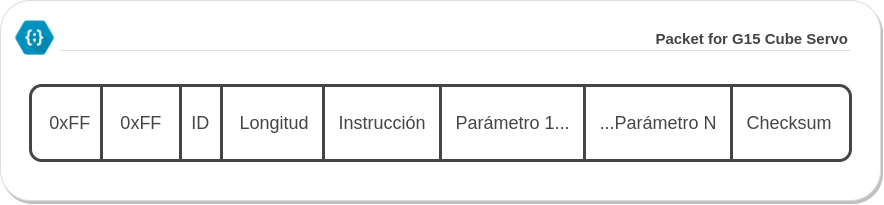
\includegraphics[width=0.9\textwidth]{figuras/Imagenes_SW/Packet_G15.png}   
    	\caption{Paquete de información genérico para comunicar con los Servos G15 Cube}
    	\label{fig:app:registrosg15:comunicacion_mensaje}
    \end{figure}
	

	\begin{table}[htbp]
		\centering
		\caption{Resumen de las instrucciones aceptadas por los Cytron G15 Cube servo}
		\label{tab:g15_instructions}
		\begin{center}
			\begin{tabular}{|c|c|c|}
			\hline
			\textbf{Instrucción} & \textbf{Valor Hex.} & \textbf{Comentarios} \\
			\hline
			iPING & 0x01 & Solicita un paquete con el estado del servo \\
			\hline
			iREAD\_DATA & 0x02 & Lee información de la memoria del servo \\
			\hline
			iWRITE\_DATA & 0x03 & Escribe información en la memoria del servo \\
			\hline
			iREG\_WRITE & 0x04 & Escribe sobre la memoria y hasta que llega la acción \ingles{ACTION} para ejecutar dichos cambios \\
			\hline
			iACTION & 0x05 & Activa la acción codificada con la instrucción \ingles{REG\_WRITE} \\
			\hline
			iRESET & 0x06 & Resetea la memoria a los valores por defecto \\
			\hline
			iSYNC\_WRITE & 0x83 & Para escribir simultáneamente información sobre varios servos \\
			\hline
			\end{tabular}
		\end{center}
	\end{table}	
	
	La respuesta por parte de los servos tiene también una estructura general que se detalla a continuación byte a byte:
	\begin{itemize}
		\item Bytes 0 y 1 de encabezado. Igual que en el caso anterior.
		\item Byte 2: codifica el ID del servo que responde.
		\item Byte 3: codifica la longitud a leer.
		\item Byte 4: sirve para informar de posibles errores en el servo. Cada bit del byte codifica un tipo de error, estando todos a 0 cuando la comunicación y el servo se encuentran buen estado. Estos errores están detallados en la tabla \ref{tab:g15_error}, junto a la máscara en binario que se aplicará a dicho byte para comprobar cada error.
		\item Bytes del 5 al N: Parámetros que envía el servo.
		\item Byte N+1: \ingles{CheckSum}.
	\end{itemize}
	
	 En la figura \ref{fig:app:registrosg15:comunicacion_mensaje_from_servo} se puede ver representado, a modo de resumen gráfico, este esquema de información genérico que se ha expuesto previamente.	
	 
	 \begin{figure}[H]
	    	\centering
	    	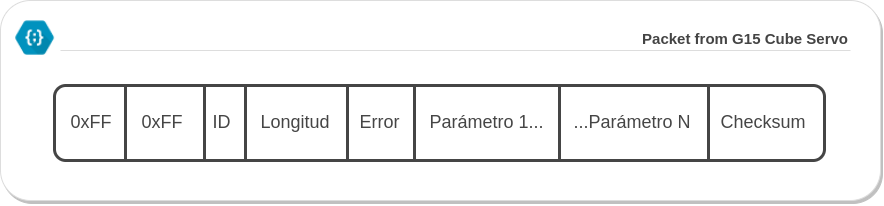
\includegraphics[width=0.9\textwidth]{figuras/Imagenes_SW/Packet_From_G15.png}   
	    	\caption{Paquete de información genérico de retorno de los Servos G15 Cube}
	    	\label{fig:app:registrosg15:comunicacion_mensaje_from_servo}
	 \end{figure}
	
	\begin{table}[htbp]
		\centering
		\caption{Codificación del error de los servos G15 Cube en cada bit del byte de error.}
		\label{tab:g15_error}
		\begin{center}
			\begin{tabular}{|c|c|c|}
				\hline
				\textbf{Bit} & \textbf{Error} & \textbf{Máscara a aplicar} \\
				\hline
				0 & Error en voltaje de entrada & 0X0001 \\
				\hline
				1 & Límite de ángulo & 0X0002 \\
				\hline
				2 & Sobrecalentamiento & 0X0004 \\
				\hline
				3 & Error en el rango pedido & 0X0008 \\
				\hline
				4 & Error en el \ingles{CheckSum} & 0X0010 \\
				\hline
				5 & Sobrecarga & 0X0020 \\
				\hline
				6 & Instrucción incorrecta & 0X0040 \\
				\hline
				7 & - & -  \\
				\hline
			\end{tabular}
		\end{center}
	\end{table}
	
	Aunque como se ha visto anteriormente y se ha detallado en la tabla \ref{tab:g15_error} el servo devuelve un solo byte de error, al leer la información recibida el error, tanto en la librería de Cytron como en la estructura desarrollada para este proyecto este byte se amplia a dos bytes para añadir la posibilidad de nuevos errores en la recepción del paquete de datos. Se pueden ver de forma detallada en la tabla \ref{tab:g15_error_second}, nuevamente junto a la máscara que se aplicará a dicho byte para cada caso. En el byte más bajo queda la información que devuelve el servo y en el más alto la información añadida.
	\\ 
	
	\begin{table}[htbp]
		\centering
		\caption{Codificación del error de comunicación en cada bit del segundo byte de error.}
		\label{tab:g15_error_second}
		\begin{center}
			\begin{tabular}{|c|c|c|}
				\hline
				\textbf{Bit} & \textbf{Error} & \textbf{Máscara a aplicar} \\
				\hline
				8 & Paquete perdido o tiempo de espera superado & 0X0100 \\
				\hline
				9 & Encabezado incorrecto & 0X0200 \\
				\hline
				10 & ID incorrecto & 0X0400 \\
				\hline
				11 & Error en el \ingles{CheckSum} & 0X0800 \\
				\hline
				12 & - & -  \\
				\hline
				13 & - & -  \\
				\hline
				14 & - & -  \\
				\hline
				15 & - & -  \\
				\hline
			\end{tabular}
		\end{center}
	\end{table}
	\section{Distintos tipos de instrucciones}
	A continuación se detallan las distintas instrucciones que aceptan los Servos, presentadas en la tabla \ref{tab:g15_instructions}.
	\subsection{Petición del estado del servo}
	
	Se hace una petición del estado o una operación de tipo \ingles{PING} cuando se quiere conocer la existencia y estado de un servo con un ID específico. Adicionalmente si se envía utilizando el ID comodín (0xFE, para todos los servos) se podrá recoger el ID del servo conectado (cuando solo haya uno).
	\\ 
	
	Un paquete para una operación \ingles{PING} podría tener el siguiente aspecto (\ingles{iPING} al servo con ID 1. El mensaje enviado tendrá una longitud de dos bytes a leer. Las diferentes instrucciones se han visto en la tabla \ref{tab:g15_instructions}):
	\begin{center}
		\begin{tabular}{|c|c|c|c|c|c|}
			\hline
			0xFF & 0xFF & 0x01 & 0x02 & 0x01 & 0xFB \\
			\hline
		\end{tabular}
	\end{center}
	
	Como se puede ver este mensaje no lleva parámetros.
	\\ 
	
	El mensaje de retorno podría ser, por ejemplo el siguiente. Respondiendo el servo con ID 1 dos bytes a leer, el error que es 0 (todo correcto) y el \ingles{CheckSum}:
	\begin{center}
		\begin{tabular}{|c|c|c|c|c|c|}
			\hline
			0xFF & 0xFF & 0x01 & 0x02 & 0x00 & 0xFC \\
			\hline
		\end{tabular}
	\end{center}
	
	\subsection{Operaciones de lectura} 
	
	Las operaciones de lectura, con la instrucción \ingles{iREAD\_DATA} vista en la tabla \ref{tab:g15_instructions} están pensadas para leer la memoria interna de los servos. Los parámetros enviados serán la dirección de memoria a partir de la cual se quiere leer y el número de bytes a leer. Se puede ver en la tabla \ref{tab:g15_register} las posibles direcciones de memoria a las que acceder, el tipo de acceso que tienen (lectura/escritura o ambos) así como los valores típicos (por defecto, máximos y mínimos).
	\\ 
	
	Un ejemplo de este tipo de mensajes puede ser una petición de lectura de la temperatura (0x2B en la tabla \ref{tab:g15_register}). En este caso sobre el servo con ID 1. La temperatura ocupa un solo byte.
		
	\begin{center}
		\begin{tabular}{|c|c|c|c|c|c|c|c|}
			\hline
			0xFF & 0xFF & 0x01 & 0x04 & 0x02 & 0x2B & 0x01 & 0xCC \\
			\hline
		\end{tabular}
	\end{center}
	
	Como en el caso anterior el paquete de retorno devolverá el ID del servo que responde, la longitud, que en este caso será de 3 bytes, y el error, el parámetro leido (un byte con la temperatura) y el \ingles{CheckSum}:
	
	\begin{center}
		\begin{tabular}{|c|c|c|c|c|c|c|}
			\hline
			0xFF & 0xFF & 0x01 & 0x03 & 0x00 & 0x20 & 0xDB \\
			\hline
		\end{tabular}
	\end{center}
	
	\subsection{Operaciones de escritura} \label{subsec:registros:operaciones:escritura}
	
	Las operaciones de escritura tienen un funcionamiento análogo al de lectura. La instrucción \ingles{iWRITE\_DATA} vista en la tabla \ref{tab:g15_instructions} envía una cadena de bytes a escribir a partir de una dirección de memoria dada. Nuevamente se pueden ver las direcciones de memoria en la tabla \ref{tab:g15_register}.
	\\ 
	
	Como ejemplo se escribirá, sobre el servo con ID 1 un ángulo objetivo (empieza en la dirección 0x1E). Como se puede ver ocupa dos bytes, empezando por el de más bajo y a continuación el más alto. A la hora de enviar el mensaje hay que tener en cuenta estos aspectos para que los parámetros vayan ordenados de igual manera:
	
	\begin{center}
		\begin{tabular}{|c|c|c|c|c|c|c|c|c|}
			\hline
			0xFF & 0xFF & 0x01 & 0x05 & 0x03 & 0x1E & 0xAA & 0x00 &0x2E  \\
			\hline
		\end{tabular}
	\end{center}
	
	El paquete de retorno en este caso devolverá el posible error en la comunicación, sin parámetros.
	\begin{center}
		\begin{tabular}{|c|c|c|c|c|c|}
			\hline
			0xFF & 0xFF & 0x01 & 0x02 & 0x00 & 0xFC \\
			\hline
		\end{tabular}
	\end{center}
	
	\subsection{Operaciones de escritura con activación desacoplada}
		
		La idea de este tipo de operación es la de enviar a distintos servos operaciones de escritura pero que queden pendientes de ejecutarse. De esta forma, utilizando la instrucció \ingles{iACTION} se podrán activar todos a la vez.
		\\ 
		
		Para la operación de escritura en memoria se seguirá un formáto análogo al descrito en el apartado \ref{subsec:registros:operaciones:escritura}. El único cambio es que la instrucción utilizada, en vez de ser \ingles{iWRITE\_DATA} como se ha descrito en dicho apartado, se utilizará la instrucción \ingles{iREG\_WRITE} (se puede consultar en la tabla \ref{tab:g15_instructions}).
		\\ 
		
		Una vez enviada la información a escribir a todos los servos, se procederá a enviar el mensaje de activación. En este caso se enviará a todos los servos conectados (ID genérico de 0xFE):
		\begin{center}
			\begin{tabular}{|c|c|c|c|c|c|}
				\hline
				0xFF & 0xFF & 0xFE & 0x02 & 0x05 & 0xFA \\
				\hline
			\end{tabular}
		\end{center}
		
		Por norma general, en los casos en los que se utiliza el ID genérico (menos en el caso de la instrucción \ingles{iPING} en los que hay un servo conectado) no se recogerá mensaje de retorno alguno.
		
	\subsection{Resetear la memoria de los servos a los valores de fábrica}
	
		La instrucción \ingles{iRESET} devolverá la memoria al estado por defecto. Se pueden ver los valores por defecto en la tabla \ref{tab:g15_register}.
		\\
		
		Para efectuarla se enviará dicha instrucción al servo correspondiente, en este caso al servo cuyo ID es 0:
		\begin{center}
			\begin{tabular}{|c|c|c|c|c|c|}
				\hline
				0xFF & 0xFF & 0x00 & 0x02 & 0x06 & 0xF7 \\
				\hline
			\end{tabular}
		\end{center}
		
		 Nuevamente el mensaje de error contendrá unicamente el posible error en la comunicación.
		 \begin{center}
		 	\begin{tabular}{|c|c|c|c|c|c|}
		 		\hline
		 		0xFF & 0xFF & 0x00 & 0x02 & 0x00 & 0xFD \\
		 		\hline
		 	\end{tabular}
		 \end{center}
		 
		 Se debe tener en cuenta, que aunque el mensaje de retorno responda con el valor inicial, una vez ejecutado el reset de la memoria el ID del servo valdrá 1 y el \ingles{baud rate} será de $19.2kb/s$
	
	\subsection{Operaciones de escritura sobre múltiples servos}
	
	\subsection{Aspectos interesantes a tener en cuenta}
		\completarCon{Cambiar de wheel mode a no wheel mode, control de velocidad que es falso, es torque lo que se pasa en wheel mode...
		¿Leer el torque que significa?}

\begin{table}[htbp]
	\caption{Características mas importantes de los Servos G15 de Cytron. Tabla traducida y resumida a los puntos más importantes del Cytron G15 Cube servo User Manual \cite{CytronTechnologies2012} \completarCon{¿esto está bien, hay que poner paginas involucradas?}}
	\label{tab:g15_register}
	\begin{adjustwidth}{-1.9cm}{-1.5cm}
	\begin{tabular}{|c|c|c|c|c|c|c|}
		\hline
		\textbf{Area} & \textbf{\shortstack{Address\\ (Hex)}} & \textbf{Parameter} & \textbf{\shortstack{Read only \\ /Read Write}} & \textbf{\shortstack{Factory\\ default\\ value (Hex)}} & \textbf{\shortstack{Minimum\\ value (Hex)}} & \textbf{\shortstack{Maximum\\ value (Hex)}} \\ \hline
		\multicolumn{ 1}{|c|}{EEPROM} & 0 (0x00) & Model (L) & R & ‘G’ (0x0F) & - & - \\ \cline{ 2- 7}
		\multicolumn{ 1}{|c|}{} & 1 (0x01) & Model(H) & R & 15 (0x47) & - & - \\ \cline{ 2- 7}
		\multicolumn{ 1}{|c|}{} & 2 (0x02) & Firmware Revision & R &  & - & - \\ \cline{ 2- 7}
		\multicolumn{ 1}{|c|}{} & 3 (0x03) & ID & RW & 1 (0x01) & 0 (0x00) & 253 (0xFD) \\ \cline{ 2- 7}
		\multicolumn{ 1}{|c|}{} & 4 (0x04) & Baud Rate & RW & 103 (0x67) & 3 (0x03) & 255 (0xFF) \\ \cline{ 2- 7}
		\multicolumn{ 1}{|c|}{} & 5 (0x05) & Return Delay & RW & 250 (0xFA)  & 1 (0x01)  & 255 (0xFF) \\ \cline{ 2- 7}
		\multicolumn{ 1}{|c|}{} & 6 (0x06) & CW Angle Limit (L) & RW & \multicolumn{ 1}{c|}{ 0 (0x0000) } & \multicolumn{ 1}{c|}{ 0 (0x0000) } & \multicolumn{ 1}{c|}{1087 (0x043F)} \\ \cline{ 2- 4}
		\multicolumn{ 1}{|c|}{} & 7 (0x07) & CW Angle Limit (H) & RW & \multicolumn{ 1}{c|}{} & \multicolumn{ 1}{c|}{} & \multicolumn{ 1}{c|}{} \\ \cline{ 2- 7}
		\multicolumn{ 1}{|c|}{} & 8 (0x08) & CCW Angle Limit (L) & RW & \multicolumn{ 1}{c|}{1087 (0x043F)} & \multicolumn{ 1}{c|}{ 0 (0x0000) } & \multicolumn{ 1}{c|}{1087 (0x043F)} \\ \cline{ 2- 4}
		\multicolumn{ 1}{|c|}{} & 9 (0x09) & CCW Angle Limit (H) & RW & \multicolumn{ 1}{c|}{} & \multicolumn{ 1}{c|}{} & \multicolumn{ 1}{c|}{} \\ \cline{ 2- 7}
		\multicolumn{ 1}{|c|}{} & 10 (0x0A) & Reserved & - & - & - & - \\ \cline{ 2- 7}
		\multicolumn{ 1}{|c|}{} & 11 (0x0B) & Temperature Limit & RW & 70 (0x46) & 0 (0x00) &  \\ \cline{ 2- 7}
		\multicolumn{ 1}{|c|}{} & 12 (0x0C) & Lowest Voltage Limit & RW & 65 (0x41) & 65 (0x41) & 178 (0xB2) \\ \cline{ 2- 7}
		\multicolumn{ 1}{|c|}{} & 13 (0x0D) & Highest Voltage Limit & RW & 150 (0x96)  &  &  \\ \cline{ 2- 7}
		\multicolumn{ 1}{|c|}{} & 14 (0x0E) & Max Torque (L) & RW & \multicolumn{ 1}{c|}{1023 (0x03FF)} & \multicolumn{ 1}{c|}{ 0 (0x0000) } & \multicolumn{ 1}{c|}{1023 (0x03FF)} \\ \cline{ 2- 4}
		\multicolumn{ 1}{|c|}{} & 15 (0x0F) & Max Torque (H) & RW & \multicolumn{ 1}{c|}{} & \multicolumn{ 1}{c|}{} & \multicolumn{ 1}{c|}{} \\ \cline{ 2- 7}
		\multicolumn{ 1}{|c|}{} & 16 (0x10) & Return Packet Enable & RW & 2 (0x02) & 0 (0x00) & 2 (0x02) \\ \cline{ 2- 7}
		\multicolumn{ 1}{|c|}{} & 17 (0x11) & Alarm LED & RW & 36 (0x24) & 0 (0x00) & 127 (0x7F) \\ \cline{ 2- 7}
		\multicolumn{ 1}{|c|}{} & 18 (0x12) & Alarm Shutdown & RW & 36 (0x24) & 0 (0x00) & 127 (0x7F) \\ \cline{ 2- 7}
		\multicolumn{ 1}{|c|}{} & 19 (0x13) & Reserved & - & - & - & - \\ \cline{ 2- 7}
		\multicolumn{ 1}{|c|}{} & 20 (0x14) & Down Calibration (L) & R &  &  &  \\ \cline{ 2- 7}
		\multicolumn{ 1}{|c|}{} & 21 (0x15) & Down Calibration (H) & R &  &  &  \\ \cline{ 2- 7}
		\multicolumn{ 1}{|c|}{} & 22 (0x16) & Up Calibration (L) & R &  &  &  \\ \cline{ 2- 7}
		\multicolumn{ 1}{|c|}{} & 23 (0x17) & Up Calibration (H) & R &  &  &  \\ \hline
		\multicolumn{ 1}{|c|}{RAM} & 24 (0x18) & Torque Enable & RW & 0 (0x00) & 0 (0x00) & 1 (0x01) \\ \cline{ 2- 7}
		\multicolumn{ 1}{|c|}{} & 25 (0x19) & LED & RW & 0 (0x00) & 0 (0x00) & 1 (0x01) \\ \cline{ 2- 7}
		\multicolumn{ 1}{|c|}{} & 26 (0x1A) & CW Compliance Margin & RW & 1 (0x01) & 0 (0x00) & 254(0xFE) \\ \cline{ 2- 7}
		\multicolumn{ 1}{|c|}{} & 27 (0x1B) & CCW Compliance & RW & 1 (0x01) & 0 (0x00) & 254(0xFE) \\ \cline{ 2- 7}
		\multicolumn{ 1}{|c|}{} & 28 (0x1C) & CW Compliance Slope & RW & 32 (0x0020) & 1 (0x01) & 254(0xFE) \\ \cline{ 2- 7}
		\multicolumn{ 1}{|c|}{} & 29 (0x1D) & CCW Compliance Slope & RW & 32 (0x0020) & 1 (0x01) & 254(0xFE) \\ \cline{ 2- 7}
		\multicolumn{ 1}{|c|}{} & 30 (0x1E) & Goal Position (L) & RW & Address 36 & \multicolumn{ 1}{c|}{ 0 (0x0000) } & \multicolumn{ 1}{c|}{1087 (0x043F)} \\ \cline{ 2- 5}
		\multicolumn{ 1}{|c|}{} & 31 (0x1F) & Goal Position (H) & RW & Address 37 & \multicolumn{ 1}{c|}{} & \multicolumn{ 1}{c|}{} \\ \cline{ 2- 7}
		\multicolumn{ 1}{|c|}{} & 32 (0x020) & Moving Speed (L) & RW & \multicolumn{ 1}{c|}{ 0 (0x0000) } & \multicolumn{ 1}{c|}{ 0 (0x0000) } & \multicolumn{ 1}{c|}{1023 (0x03FF)} \\ \cline{ 2- 4}
		\multicolumn{ 1}{|c|}{} & 33 (0x21) & Moving Speed (H) & RW & \multicolumn{ 1}{c|}{} & \multicolumn{ 1}{c|}{} & \multicolumn{ 1}{c|}{} \\ \cline{ 2- 7}
		\multicolumn{ 1}{|c|}{} & 34 (0x22) & Torque Limit (L) & RW & Address 14 & \multicolumn{ 1}{c|}{ 0 (0x0000) } & \multicolumn{ 1}{c|}{1023 (0x03FF)} \\ \cline{ 2- 5}
		\multicolumn{ 1}{|c|}{} & 35 (0x23) & Torque Limit (H) & RW & Address 15 & \multicolumn{ 1}{c|}{} & \multicolumn{ 1}{c|}{} \\ \cline{ 2- 7}
		\multicolumn{ 1}{|c|}{} & 36 (0x24) & Present Position (L) & R & \multicolumn{ 1}{c|}{} & \multicolumn{ 1}{c|}{} & \multicolumn{ 1}{c|}{} \\ \cline{ 2- 4}
		\multicolumn{ 1}{|c|}{} & 37 (0x25) & Present Position (H) & R & \multicolumn{ 1}{c|}{} & \multicolumn{ 1}{c|}{} & \multicolumn{ 1}{c|}{} \\ \cline{ 2- 7}
		\multicolumn{ 1}{|c|}{} & 38 (0x26) & Present Speed (L) & R & \multicolumn{ 1}{c|}{} & \multicolumn{ 1}{c|}{} & \multicolumn{ 1}{c|}{} \\ \cline{ 2- 4}
		\multicolumn{ 1}{|c|}{} & 39 (0x27) & Present Speed (H) & R & \multicolumn{ 1}{c|}{} & \multicolumn{ 1}{c|}{} & \multicolumn{ 1}{c|}{} \\ \cline{ 2- 7}
		\multicolumn{ 1}{|c|}{} & 40 (0x28) & Present Load (L) & R & \multicolumn{ 1}{c|}{} & \multicolumn{ 1}{c|}{} & \multicolumn{ 1}{c|}{} \\ \cline{ 2- 4}
		\multicolumn{ 1}{|c|}{} & 41 (0x29) & Present Load (H) & R & \multicolumn{ 1}{c|}{} & \multicolumn{ 1}{c|}{} & \multicolumn{ 1}{c|}{} \\ \cline{ 2- 7}
		\multicolumn{ 1}{|c|}{} & 42 (0x2A) & Present Voltage & R &  &  &  \\ \cline{ 2- 7}
		\multicolumn{ 1}{|c|}{} & 43 (0x2B) & Present Temperature & R &  &  &  \\ \cline{ 2- 7}
		\multicolumn{ 1}{|c|}{} & 44 (0x2C) & Registered & R & 0 (0x00) & 0 (0x00) & 1 (0x01) \\ \cline{ 2- 7}
		\multicolumn{ 1}{|c|}{} & 45 (0x2D) & Reserved & - & - & - & - \\ \cline{ 2- 7}
		\multicolumn{ 1}{|c|}{} & 46 (0x2E) & Moving & R & 0 (0x00) & 0 (0x00) & 1 (0x01) \\ \cline{ 2- 7}
		\multicolumn{ 1}{|c|}{} & 47 (0x2F) & Lock & RW & 0 (0x00) & 1 (0x01) & 1 (0x01) \\ \cline{ 2- 7}
		\multicolumn{ 1}{|c|}{} & 48 (0x30) & Punch (L) & RW & \multicolumn{ 1}{c|}{32 (0x0020)} & \multicolumn{ 1}{c|}{0 (0x0000)} & \multicolumn{ 1}{c|}{1023 (0x03FF)} \\ \cline{ 2- 4}
		\multicolumn{ 1}{|c|}{} & 49 (0x31) & Punch (H) & RW & \multicolumn{ 1}{c|}{} & \multicolumn{ 1}{c|}{} & \multicolumn{ 1}{c|}{} \\ \hline
	\end{tabular}
\end{adjustwidth}
\end{table}	


	
	\chapter{Protocolo de comunicación del brazo robótico} \label{app:comunicacion_brazo}
		\hrule
		\vspace{3mm}
		\completarCon{TBD una vez esté implementado}
	
	\chapter{Documentación del software} \label{app:documentacion_software}
		\hrule
		\vspace{3mm}
		%\include{doxygen_documentation/refman}
%\input{doxygen_documentation/refman}






%\end{appendices}
